\documentclass[12pt,a4paper]{article}
\usepackage[english]{babel}
\usepackage[T1]{fontenc}
\usepackage{graphicx}
\usepackage{hyperref} % \hypersetup{hidelinks=true}  % avoid colored box in links
\usepackage{multirow}
\usepackage{tabularx}

% redefine the X column to be based on a m-column instead of a p-column
\renewcommand\tabularxcolumn[1]{m{#1}}

\usepackage{longtable}
\usepackage[table]{xcolor}
\usepackage{fancyhdr}
\usepackage{lipsum}

\usepackage{tcolorbox}
% \definecolor{mycolor1}{rgb}{0.545, 0.278, 0.208}
% \definecolor{mycolor2}{rgb}{0.949, 0.949, 0.949}

% Select Arial font for the whole document
\usepackage{helvet}
\renewcommand{\familydefault}{\sfdefault}

% Document geometry
\usepackage[a4paper, includehead,
  textwidth=16cm, textheight=23cm,
  headheight=2.7cm,
  includemp,
  marginparsep=0.cm,
  marginparwidth=0.cm,
  %showframe,
]{geometry}

\usepackage{enumerate}
\usepackage[shortlabels]{enumitem}
\usepackage{tocloft}

% AD and RD entries
\newenvironment{ADlist}
               {\begin{enumerate}[start=1,label={AD\arabic*}]}  % \bfseries
               {\end{enumerate}}               
\newenvironment{RDlist}
               {\begin{enumerate}[start=1,label={RD\arabic*}]}  % \bfseries
               {\end{enumerate}}
\newcommand{\ARDitem}[2]{\item \label{#1} {#2}}
\newcommand{\citedoc}[1]{[\ref{#1}]}


% List of requirements
\newcommand{\listreqname}{List of Requirements:}
\newlistof{req}{toreq}{\listreqname}
\newcommand{\req}[2]{%
\refstepcounter{req}
\par\vspace{0.2cm}\noindent\textbf{\ESOreqprefix{}\thereq:} #2 \label{#1}\vspace{0.2cm}
\addcontentsline{toreq}{req}
{\protect \textbf{\ESOreqprefix{}\numberline{\thereq}}#2}\par}
\newcommand{\citereq}[1]{\textbf{\ESOreqprefix{}\ref{#1}}}


% List of questions
\newcommand{\listquestionname}{List of Questions:}
\newlistof{question}{toquestion}{\listquestionname}
\newcommand{\question}[2]{%
\refstepcounter{question}
\par\vspace{0.2cm}\noindent\textbf{Q\thequestion:} #2 \label{#1}\vspace{0.2cm}
\addcontentsline{toquestion}{question}
{\protect \textbf{Q\numberline{\thequestion}}#2}\par}
\newcommand{\citequestion}[1]{\textbf{Q\ref{#1}}}


% ====================================================================
% Document properties
%
\newcommand{\ESOdoctitle}{CUBES Document Title}
\newcommand{\ESOdocnumber}{CUBES-123-456-789}
\newcommand{\ESOdocversion}{0.1}
\newcommand{\ESOdoctype}{Specification}
\newcommand{\ESOdocstatus}{Draft}  % Released
\newcommand{\ESOdocorganization}{CUBES Consortium}
\newcommand{\ESOdocreleasedate}{2023-12-31}
\newcommand{\ESOdocclassification}{CUBES Consortium Internal\newline[Confidential for non-CUBES staff]}
\newcommand{\ESOreqprefix}{R-CUB-}
\newcommand{\ESOowner}{TBD Owner}
\newcommand{\ESOapprovedby}{TBD ApprovedBy}
\newcommand{\ESOreleasedby}{TBD ReleasedBy}

\begin{document}
% ====================================================================
% Running header
%
\pagestyle{fancy}
\fancyhead{} % clear all header fields
\fancyfoot{} % clear all footer fields

\fancyhead[L]{
  \begin{tabularx}{0.46\headwidth}{Xc}
    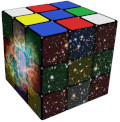
\includegraphics[width=2.2cm]{media/CUBES_logo.jpg}  &  {\small \ESOdoctitle{}}\\
  \end{tabularx}
}
\fancyhead[R]{
    \footnotesize
    \begin{tabularx}{0.48\headwidth}{|X|l|}
      \hline
        {Document number:}         &      \ESOdocnumber{}     \\\hline
        {Document version:}        &      \ESOdocversion{}    \\\hline
        {Document status:}         &      \ESOdocstatus{}     \\\hline
        {Released on:}             &      \ESOdocreleasedate  \\\hline
        {Page:}                    &      \thepage{} of \pageref{LastPage} \\\hline
    \end{tabularx}
}


% ====================================================================
% Title page
%
\thispagestyle{empty}
\newgeometry{headheight=0cm, textheight=25cm}
\begin{center}
  \begin{tabularx}{\textwidth}{|X|X|}
    \hline
        {\bf \small Document title:}          & {\bf \ESOdoctitle{}}         \\[0.8cm] \hline
        {\bf \small Document number:}         &      \ESOdocnumber{}         \\[0.8cm] \hline
        {\bf \small Document verision:}       &      \ESOdocversion{}        \\[0.8cm] \hline
        {\bf \small Document type:}           &      \ESOdoctype{}           \\[0.8cm] \hline
        {\bf \small Document status:}         &      \ESOdocstatus{}         \\[0.8cm] \hline
        {\bf \small Releasing organization:}  &      \ESOdocorganization{}   \\[0.8cm] \hline
        {\bf \small Released on:}             &      \ESOdocreleasedate      \\[0.8cm] \hline
        {\bf \small Document classification:} &      \ESOdocclassification{} \\[0.8cm] \hline
  \end{tabularx}
\end{center}

\vfill

\begin{center}
  \begin{tabularx}{\textwidth}{|l|X|c|}
    \hline
    {\bf \small Prepared by:} &  \ESOowner{}                & \hspace{0.5cm} \textcolor{gray}{Signature} \hspace{0.5cm} \ \\[0.8cm] \hline
    {\bf \small Approved by:} &  \ESOapprovedby{}           &                \textcolor{gray}{Signature}                  \\[0.8cm] \hline
    {\bf \small Released by:} &  \ESOreleasedby{}           &                \textcolor{gray}{Signature}                  \\[0.8cm] \hline
  \end{tabularx}
\end{center}


\restoregeometry



% ====================================================================
% Authors and change record
\newpage
\pagestyle{fancy}

\noindent
{\Large \bf Authors}
\medskip

\noindent
\begin{tabularx}{\textwidth}{|l|X|}
  \hline
      {\bf Name} & {\bf Affiliation}\\
      \hline
      Name Surname 1     & Institute 1 \\ \hline
      Name Surname 2     & Institute 2 \\ \hline
      ...                & ...         \\ \hline
\end{tabularx}

\vspace{3cm}

\noindent
{\Large \bf Change Record from previous versions}
\medskip

\noindent
\begin{tabularx}{\textwidth}{|l|X|}
  \hline
      {\bf Affected Section(s)} & {\bf Changes / Reason / Remarks}\\  \hline
      Sect.~\ref{sec:scope}&  Minor changes \\ \hline
\end{tabularx}


% ====================================================================
% Table of contents
\newpage
\tableofcontents \thispagestyle{fancy}


% ====================================================================
% Document contents
\newpage
\section{Introduction}
\label{sec:intro}

A brief description of the topic addressed by this document.


\section{Scope}
\label{sec:scope}

Identify target audience (to whom this document is addessed).


\subsection{Definitions, Acronyms and Abbreviations}
\label{sec:acronyms}

This document employs several abbreviations and acronyms to refer concisely to an item, after it has been introduced. The following list is aimed to help the reader in recalling the extended meaning of each short expression:

\begin{longtable}{ |l|l| }
A\&G & Acquisition and Guiding \\ \hline
ADC & Atmospheric Dispersion Corrector \\ \hline
AFC & Active Flexure Compensation (system) \\ \hline
AM & Air Mass \\ \hline
API & Application Programming Interface \\ \hline
BOB & Broker for Observation Blocks \\ \hline
CCD & Charge-Coupled Device \\ \hline
CCF & Camera Control Framework \\ \hline
CII & Core Integration Infrastructure \\ \hline
CPL & Common Pipeline Library \\ \hline
CU & Calibration Unit \\ \hline
CUBES & Cassegrain U-Band Efficient Spectrograph \\ \hline
DAS & Data Analysis Software \\ \hline
DCS & Detector Control System \\ \hline
DDT & Data Display Tool \\ \hline
DHS & Data Handling System \\ \hline
DPM & Data Product Manager \\ \hline
DRS & Data Reduction Software \\ \hline
E2E & End-to-end (simulator) \\ \hline
ELT & Extremely Large Telescope \\ \hline
ESO & European Southern Observatory \\ \hline
ETC & Exposure Time Calculator \\ \hline
ETR & Extensible Test Runner \\ \hline
FB & Function Block (PLC) \\ \hline
FCF & Function Control Framework \\ \hline
FCS & Function Control System \\ \hline
FITS & Flexible Image Transport System \\ \hline
FL & Fibre Link \\ \hline
GUI & Graphical User Interface \\ \hline
ICS & Instrument Control Software \\ \hline
IFW & Instrument Control System Framework \\ \hline
INS & Instrumentation Software \\ \hline
IWS & Instrument Workstation \\ \hline
LAN & Local Area Network \\ \hline
LCS & Local Control System (PLC) \\ \hline
LDLS & Laser Driven Light Source \\ \hline
ND & Neutral Density \\ \hline
NDIT & Number of Detector Integrations \\ \hline
NGCII & New General detector Controller II \\ \hline
OB & Observation Block \\ \hline
OCA & Organization/Classification/Association \\ \hline
OCF & Observation Coordination Framework \\ \hline
OCM & Observation Coordination Manager \\ \hline
OCS & Observation Coordination System \\ \hline
OLAS & On-Line Archive Subsystem \\ \hline
OLDB & On-Line DataBase \\ \hline
OPC-UA & Open Platform Communications-Unified Architecture \\ \hline
OPS & Observation Preparation Software \\ \hline
OT & Observing Tool \\ \hline
PLC & Programmable Logic Controller \\ \hline
PM & Project Manager \\ \hline
PSF & Point Spread Function \\ \hline
RRM & Rapid-Response Mode \\ \hline
SSE & Software System Engineer \\ \hline
TBC & To Be Confirmed \\ \hline
TBD & To Be Defined \\ \hline
TCS & Telescope Control Software \\ \hline
TRS & Technical Requirements Specification \\ \hline
TOO & Target Of Opportunity \\ \hline
TLR & Top Level Requirement \\ \hline
UVES & Ultraviolet and Visual Echelle Spectrograph \\ \hline
VLTSW & VLT SoftWare \\ \hline
VLT & Very Large Telescopes \\ \hline
vOT & visitor mode Observing Tool \\ \hline
WP & Work Package \\ \hline
WS & Workstation \\ \hline
\end{longtable}

\section{Related documents}
\label{sec:related_docs}

The following documents, of the exact version shown, form part of this document to the extent specified herein. In the event of conflict between the documents referenced herein and the content of this document, the content of this document shall be considered as superseding.  AD references shall be specific about which part of the target document is the subject of the reference.

\subsection{Applicable documents}
\label{sec:applicable_docs}

\begin{ADlist}
  \ARDitem{AD:ESO-379353}{Common Requirements for VLT Instruments;\\ESO-379353, Version 3}
  \ARDitem{AD:ESO-351071}{ICS Software Specification;\\ESO-351071, Version 1}
\end{ADlist}


\subsection{Reference documents}
\label{sec:reference_docs}

\begin{RDlist}
  \ARDitem{RD:ESO-351097}{VLT-ELT Gateway Software Design Description;\\ESO-351097, Version 2}
  \ARDitem{RD:ESO-363357}{ELT ICS Framework - Online Data Processing - User Manual;\\ESO-363357, Version 2}
  \ARDitem{RD:ESO-363358}{ELT ICS Framework - Sequencer - User Manual;\\ESO-363358, Version 1}
\end{RDlist}


\section{Main matter}

\subsection{Requirements}

\lipsum[1]

\req{req:nolights}{Switch off the lights.}

\lipsum[2]

\req{req:generic_req}{Another reuquirement.}

\subsection{Questions}

\lipsum[3]

\question{q:where}{Where is the coffee machine?}

\lipsum[4]

\question{q:when}{When is the coffee break scheduled?}


\subsection{References}

\lipsum[5]

\begin{itemize}
\item Sect.~\ref{sec:intro}, Sect.~\ref{sec:scope};
\item \citedoc{AD:ESO-379353}, \citedoc{RD:ESO-363358};
\item \citereq{req:nolights}, \citereq{req:generic_req};
\item \citequestion{q:where}, \citequestion{q:when};
\item Tab.~\ref{tab:test}, Fig.~\ref{fig:m31}, Eq.~\ref{eq:eq};
\end{itemize}


\subsection{Figures and tables}

\lipsum[6]

\begin{figure}[hbtp!]
  \centering
  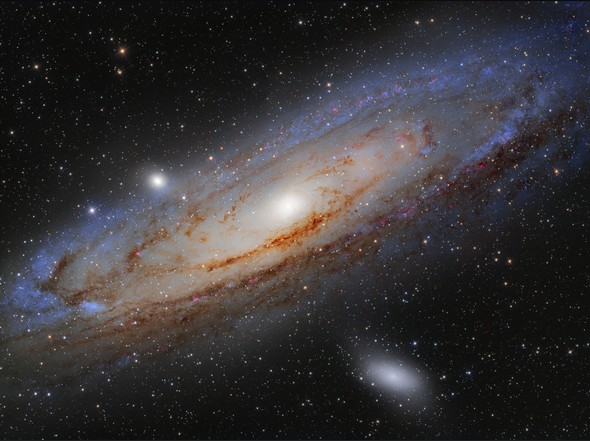
\includegraphics[width=0.5\textwidth]{media/m31}
  \caption{Andromeda galaxy}
    \label{fig:m31}
\end{figure}


\lipsum[7]

\begin{table}[hbtp!]
  \centering
  \begin{tabular}{ |l|l|l| }
    \hline
    \rowcolor{lightgray} \multicolumn{3}{|c|}{Country List} \\
    \hline
    Country Name or Area Name& ISO ALPHA 2 Code &ISO ALPHA 3 \\
    \hline
    Afghanistan & AF &AFG \\
    \rowcolor{gray}
    Aland Islands & AX & ALA \\
    Albania   &AL & ALB \\
    Algeria  &DZ & DZA \\
    American Samoa & AS & ASM \\
    Andorra & AD & \cellcolor[HTML]{AA0044} AND    \\
    Angola & AO & AGO \\
    \hline
  \end{tabular}
  \caption{Table to test captions and labels.}
  \label{tab:test}
\end{table}



% ====================================================================
% List of requirements
\newpage
\listofreq \thispagestyle{fancy}

% List of questions
\listofquestion \thispagestyle{fancy}


\label{LastPage}

\end{document}
